\chapter{Testovací program}
Testovací systém běžící na serveru testovací laboratoře se skládá z několika samostaných částí. Základem celého systému je databáze uchovávající všechna informace struktuře testovací laboratoře data s výsledky jednotlivých testů. Program testlab se stará o celý průběh testování. Několika málo přepínači lze nastavit průběh testování. Další součástí je sada programů nazývající se testovací API. Tyto programu usnadňují psaní jednotlivých testů. Nedílnou součástí testovacího systému jsou testovací skripty, které lze rozdělit na skripty pro stáhnutí projektu, kompilaci projektu, testování výrobku a úklid projektu. Poslední součástí testovacího systému je webový interface pro sledování výsledků testování a nastavování chování testovacího systému.

\section{Adresářová struktura testovacího systému}

Jednotlivé částí testovacího systému jsou rozloženy v adresářové struktuře serveru následovně. Testovací program a testovací API jsou umístěny v adresáři /usr/bin, aby byly odevšad jednoduše spustitelné. Sdílené knihovny, které využívá testovací program a mohou ho využívat nové programy testovacího API jsou umístěny v adresáři /usr/lib. Hlavičkové soubory pro tyto knihovny jsou k naleznutí v adresáři /usr/include/testlab. Tato část testovacího systému se za běhu nemění a zůstává stejná. Jednou vyjímkou je aktualizace testovacího systému, při které mohou být opraveny chyby či přidán nový program do testovacího API. Tuto aktualizaci může provádět pouze administrátor.

Druhá část adresářové struktury testovacího systému obsahuje soubory a adresáře měnící se v průběhu běhu testovacího systému. Tato část se nechází v adresáři /var/testlab a je rozdělena na následující podadresáře. Adresář clean obsahuje skripty pro zajištění úklidu po překladu jednotlivých platforem. Adresář compile obsahuje skripty zajišťující kompilaci jednotlivých výrobků všech platforem. Pro každou platformu je v tomto adresáři jeden skript a výrobek sem mu zadává jako parametr. V adresáři checkout nalezneme skripty pro stáhnutí zdrojových kódu platformy. Pro stahování zdrojových kódů se budou často využívat repozitáře a v mém systému bude konkrétně využit verzovací systém git. Project je pracovním adresářem kam jsou stahované zdrojové kódy jednotlivých platforem a kde jsou následně překládány. Dále je tento adresář rozdělen do jednotlivých podadresářů podle jednotlivých releasů překládaného firmwaru. V každém adresářy releasu jsou adresáře pro každou testovanou platformu. Adresáře jednotlivých releasu se před ukončením programu testlab mažou, jelikož dále nejsou potřeba a zabírají velký prostor na disku. Přeložený firmware všech výrobků je ukládán do adresáře firmware a do podadresáře s názevem identifikačního čísla releasu, pro který byl firmware přeložen. Firmwary se zde uchovávají většinou do vydání další verze ostrého firmwaru. Předchozí firmwary jsou zálohovány na jiný server či jiný disk testovacího serveru, pro zachování místa na systémovém ssd disku testovacího serveru. Testovací skripty se nacházejí v adresáři tests. Adresář tests se dále dělí na podadresáře s názvy testovaných funkcí, ve kterých se nacházejí jednotlivé testovací skripty jejichž název je schodný s testovací procedurou. Konfigurace nahrávané do routeru během testování jsou uloženy v adresáři conf. Adresář conf je dále rozdělen podle testovaných funkcí. V každém adresáři dané funkce jsou adresáře pojmenované podle identifikačních čísel jednotlivých routerů ve kterých se již nacházejí jednotlivé konfigurace routerů. Posledním adresářem této části testovacího systému je adresář logs. V adresáři logs se ukládají logy z jednotlivých fází testování. Ukládájí se zde logy ze stáhování zdrojových kódů, ze samotné kompilace všech výrobků a z úklidu po překladu. Adresář je členěn podle typu logu a dále podle releasu testovaného firmwaru. Logy starších releasu se stejně jako firmware přesouvají na jiný disk nebo mažou. Logy ze samotných testů se jako jediný ukládají do databáze.

\begin{figure}[h]
  \centering
  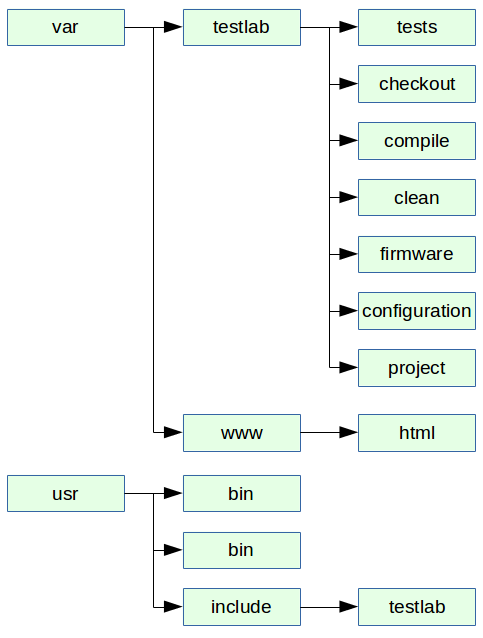
\includegraphics[width=.4\LW]{adresar_struktura}
  \caption{Adresářová struktura testovacího systému}
  \label{fig:adresar_struktura}
\end{figure}

Třetí část testovacího systému se nchází v adresáři /var/www/html. Tuto část testovacího systému tvoří samotné webové stránky testovacího systému

\section{Struktura databáze}

\section{Popis programu}

O průběh celého testu se stará program testlab. Testlab je program psaný v jazyc C. Program po spuštění otevře systémový log pro možnost logování chyb do systémového logu. Filtrováný systémový log by měl později být zobrazován na webowém rozhraní testovacího systému. První hláškou do systémového logu je informace o spuštění programu testlab, daným uživatelem a v určený čas. Po otevření systémového logu program rozebírá parametry na příkazové řádce. Parametry jsou rozebíráný pomocí funkce getopts. Pomocí parametrů lze ovlivnit chování programu testlab !!!!!DOPLNIT PARAMETRY!!!!!!

\begin{figure}[h]
  \centering
  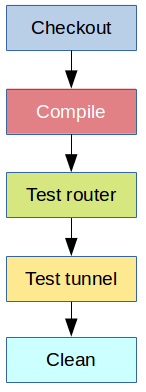
\includegraphics[width=.4\LW]{program_schema}
  \caption{Základní schéma testovacího programu}
  \label{fig:program_schema}
\end{figure}


Nyní se provádějí přípravné kroky pro samotné testování. Nejdříve je vytvořen nový release firmwaru a následně vložen do databáze. V projektovém adresáři je vytvořen nový adresář se stejným názvem jako identifikační číslo testovaného releasu.

\subsection{Checkout}
\subsection{Compile}
\subsection{Test router}
\subsection{Test tunel}
\subsection{Clean}
\subsection{Remote server}
\subsubsection{Telnet}
\subsubsection{SSH}

\endinput
